\documentclass[a4paper, 12pt]{article} % a4 is 210mm x 297mm
\usepackage[dvipsnames]{xcolor}
\usepackage{listings}
\usepackage{graphicx}
\usepackage{tikz}
\usepackage{fancyvrb}
\usepackage{hyperref}
\usepackage{sectsty}
\lstset { %
    language=C++
}

\allsectionsfont{\centering}

% redefine \VerbatimInput
\RecustomVerbatimCommand{\VerbatimInput}{VerbatimInput}%
{fontsize=\footnotesize,
 %
 frame=lines,  % top and bottom rule only
 framesep=2em, % separation between frame and text
 rulecolor=\color{Gray},
 %
%  label=\fbox{\color{Black}data.txt},
 labelposition=topline,
 %
 commandchars=\|\(\), % escape character and argument delimiters for
                      % commands within the verbatim
 commentchar=*        % comment character
}

\title{Using Pseudo-Random Numbers Repeatably in a Fine-Grain Multithreaded Simulation}
\author{Dmitry Savin}
\date{\today}

\usepackage[utf8]{inputenc}

\newcommand{\MD}{Merkle-Damg\r{a}rd}

\begin{document}
 \maketitle

 \section*{ Motivation }
  Particle transport Monte Carlo simulations are a key tool for High Energy Physics experiments, including the LHC experiments at CERN.
  All Monte Carlo (MC) simulations depend vitally on Pseudo-Random Number Generators (PRNGs) used to sample many distributions.
  PRNGs used must possess very large periods, fast execution, the ability to create a large number of streams, and very good correlation properties between streams and sampled values. It must be possible to reproduce a simulated event any time, for reexamination or debugging.

  Because of the transition from event-level parallelism in Geant4 to dynamical multithreading in GeantV, the tracks in one event or even parts of the same track are processed by different threads.
  Thus to assure reproducibility the pseudo-random engine state must be associated with the track itself;
  and the state of the secondary track has to be a deterministic function of the parent track.
  The state can be initialized by seeding the generator with the hashed pedigree of the track.
  
 \section*{ Goals }
 
  \begin{itemize}
   \item Implement a standalone prototype to demonstrate deterministic random number generation independent of invocation order.
   \item Associate additional PRNG information with tracks in Geant4 for reproducible simulation.
   \item Add generators with substreaming capability.
   \item Test reproducibility with different track processing order.
   \item Profile the overhead of setting the generator state.
   \item Benchmark the new generators.
  \end{itemize}
  
 \section*{ Implementation }
 
  \subsection*{ Standalone prototype }
   The standalone prototype was implemented in accordance with the \href{https://sd57.github.io/g4dprng/gsoc-proposal-Savin.html}{proposal}.
   There is an implementation compatible with any HepRandomEngine from the CLHEP library included in geant4
   and a specific version for Philox and Threefry generators from
   \href{https://www.deshawresearch.com/resources_random123.html}{Random123} library
   to reduce the abstraction overhead.
   There is a unit test for each implementation that traverses the tree in width-first and depth-first order and checks the equality of outcome.

   \subsection*{ Geant4-based prototype }
   
  \begin{figure}
   \scalebox{.5}{\setlength{\unitlength}{4144sp}%
%
\begingroup\makeatletter\ifx\SetFigFont\undefined%
\gdef\SetFigFont#1#2#3#4#5{%
  \reset@font\fontsize{#1}{#2pt}%
  \fontfamily{#3}\fontseries{#4}\fontshape{#5}%
  \selectfont}%
\fi\endgroup%
\begin{picture}(12708,5958)(397,-7315)
{\color[rgb]{0,0,0}\thicklines
\put(6751,-4178){\circle*{224}}
}%
{\color[rgb]{0,0,0}\put(6751,-6878){\circle*{224}}
}%
{\color[rgb]{0,0,0}\put(6751,-6203){\circle*{224}}
}%
{\color[rgb]{0,0,0}\put(6751,-5528){\circle*{224}}
}%
{\color[rgb]{0,0,0}\put(6751,-4853){\circle*{224}}
}%
{\color[rgb]{0,0,0}\put(6751,-3503){\circle*{224}}
}%
{\color[rgb]{0,0,0}\put(6751,-2828){\circle*{224}}
}%
\put(3181,-3612){\makebox(0,0)[lb]{\smash{{\SetFigFont{20}{24.0}{\rmdefault}{\bfdefault}{\updefault}{\color[rgb]{0,0,0}1}%
}}}}
\put(3061,-3496){\makebox(0,0)[lb]{\smash{{\SetFigFont{20}{24.0}{\rmdefault}{\bfdefault}{\updefault}{\color[rgb]{0,0,0}i}%
}}}}
\put(4861,-3496){\makebox(0,0)[lb]{\smash{{\SetFigFont{20}{24.0}{\rmdefault}{\bfdefault}{\updefault}{\color[rgb]{0,0,0}i}%
}}}}
\put(4981,-3612){\makebox(0,0)[lb]{\smash{{\SetFigFont{20}{24.0}{\rmdefault}{\bfdefault}{\updefault}{\color[rgb]{0,0,0}2}%
}}}}
\put(8461,-3496){\makebox(0,0)[lb]{\smash{{\SetFigFont{20}{24.0}{\rmdefault}{\bfdefault}{\updefault}{\color[rgb]{0,0,0}i}%
}}}}
\put(8581,-3612){\makebox(0,0)[lb]{\smash{{\SetFigFont{20}{24.0}{\rmdefault}{\bfdefault}{\updefault}{\color[rgb]{0,0,0}n}%
}}}}
{\color[rgb]{0,0,0}\put(11453,-4786){\oval(1574,900)}
}%
{\color[rgb]{0,0,0}\put(11431,-5911){\vector( 0, 1){720}}
}%
{\color[rgb]{0,0,0}\put(10666,-7261){\framebox(1575,1350){}}
}%
\put(10891,-6361){\makebox(0,0)[lb]{\smash{{\SetFigFont{20}{24.0}{\rmdefault}{\bfdefault}{\updefault}{\color[rgb]{0,0,0}hashed}%
}}}}
\put(10801,-6991){\makebox(0,0)[lb]{\smash{{\SetFigFont{20}{24.0}{\rmdefault}{\bfdefault}{\updefault}{\color[rgb]{0,0,0}pedigree}%
}}}}
\put(10801,-4921){\makebox(0,0)[lb]{\smash{{\SetFigFont{20}{24.0}{\rmdefault}{\bfdefault}{\updefault}{\color[rgb]{0,0,0}set seed}%
}}}}
{\color[rgb]{0,0,0}\put(4951,-6586){\oval(1350,1350)}
}%
{\color[rgb]{0,0,0}\put(4951,-4914){\oval(900,644)}
}%
{\color[rgb]{0,0,0}\put(8551,-4914){\oval(900,644)}
}%
{\color[rgb]{0,0,0}\put(8551,-6586){\oval(1350,1350)}
}%
{\color[rgb]{0,0,0}\put(3151,-6586){\oval(1350,1350)}
}%
{\color[rgb]{0,0,0}\put(3151,-4898){\oval(900,676)}
}%
{\color[rgb]{0,0,0}\put(1801,-6586){\vector( 1, 0){675}}
}%
{\color[rgb]{0,0,0}\put(3826,-6586){\vector( 1, 0){450}}
}%
{\color[rgb]{0,0,0}\put(6976,-6586){\vector( 1, 0){900}}
}%
{\color[rgb]{0,0,0}\put(9226,-6586){\vector( 1, 0){1440}}
}%
{\color[rgb]{0,0,0}\put(4951,-5279){\vector( 0,-1){643}}
}%
{\color[rgb]{0,0,0}\put(8551,-5279){\vector( 0,-1){643}}
}%
{\color[rgb]{0,0,0}\put(3151,-5279){\vector( 0,-1){643}}
}%
{\color[rgb]{0,0,0}\put(3151,-3886){\vector( 0,-1){675}}
}%
{\color[rgb]{0,0,0}\put(4951,-3886){\vector( 0,-1){675}}
}%
{\color[rgb]{0,0,0}\put(8551,-3886){\vector( 0,-1){675}}
}%
{\color[rgb]{0,0,0}\put(3151,-2311){\vector( 0,-1){675}}
}%
{\color[rgb]{0,0,0}\put(4951,-2311){\vector( 0,-1){675}}
}%
{\color[rgb]{0,0,0}\put(8551,-2311){\vector( 0,-1){675}}
}%
{\color[rgb]{0,0,0}\put(4501,-3843){\framebox(900,857){}}
}%
{\color[rgb]{0,0,0}\put(2701,-2268){\framebox(6300,857){}}
}%
{\color[rgb]{0,0,0}\put(8101,-3843){\framebox(900,857){}}
}%
{\color[rgb]{0,0,0}\put(2701,-3843){\framebox(900,857){}}
}%
{\color[rgb]{0,0,0}\put(451,-7261){\framebox(1350,1350){}}
}%
{\color[rgb]{0,0,0}\put(9901,-3886){\framebox(3150,2475){}}
}%
{\color[rgb]{0,0,0}\multiput(9901,-2536)(-344.11765,0.00000){26}{\line(-1, 0){172.059}}
\multiput(1126,-2536)(0.00000,-355.26316){10}{\line( 0,-1){177.632}}
\put(1126,-5911){\vector( 0,-1){0}}
}%
{\color[rgb]{0,0,0}\put(5626,-6586){\vector( 1, 0){900}}
}%
{\color[rgb]{0,0,0}\put(11431,-4291){\vector( 0, 1){450}}
}%
\put(541,-6361){\makebox(0,0)[lb]{\smash{{\SetFigFont{20}{24.0}{\rmdefault}{\bfdefault}{\updefault}{\color[rgb]{0,0,0}random}%
}}}}
\put(676,-7036){\makebox(0,0)[lb]{\smash{{\SetFigFont{20}{24.0}{\rmdefault}{\bfdefault}{\updefault}{\color[rgb]{0,0,0}seeds}%
}}}}
\put(2611,-6631){\makebox(0,0)[lb]{\smash{{\SetFigFont{14}{16.8}{\rmdefault}{\bfdefault}{\updefault}{\color[rgb]{0,0,0}combine}%
}}}}
\put(4411,-6631){\makebox(0,0)[lb]{\smash{{\SetFigFont{14}{16.8}{\rmdefault}{\bfdefault}{\updefault}{\color[rgb]{0,0,0}combine}%
}}}}
\put(8011,-6631){\makebox(0,0)[lb]{\smash{{\SetFigFont{14}{16.8}{\rmdefault}{\bfdefault}{\updefault}{\color[rgb]{0,0,0}combine}%
}}}}
\put(2881,-5011){\makebox(0,0)[lb]{\smash{{\SetFigFont{14}{16.8}{\rmdefault}{\bfdefault}{\updefault}{\color[rgb]{0,0,0}hash}%
}}}}
\put(4681,-5011){\makebox(0,0)[lb]{\smash{{\SetFigFont{14}{16.8}{\rmdefault}{\bfdefault}{\updefault}{\color[rgb]{0,0,0}hash}%
}}}}
\put(8281,-5011){\makebox(0,0)[lb]{\smash{{\SetFigFont{14}{16.8}{\rmdefault}{\bfdefault}{\updefault}{\color[rgb]{0,0,0}hash}%
}}}}
\put(4591,-1951){\makebox(0,0)[lb]{\smash{{\SetFigFont{34}{40.8}{\rmdefault}{\bfdefault}{\updefault}{\color[rgb]{0,0,0}pedigree}%
}}}}
\put(10351,-2311){\makebox(0,0)[lb]{\smash{{\SetFigFont{34}{40.8}{\rmdefault}{\bfdefault}{\updefault}{\color[rgb]{0,0,0}random}%
}}}}
\put(10126,-3436){\makebox(0,0)[lb]{\smash{{\SetFigFont{34}{40.8}{\rmdefault}{\bfdefault}{\updefault}{\color[rgb]{0,0,0}generator}%
}}}}
\put(10351,-2851){\makebox(0,0)[lb]{\smash{{\SetFigFont{34}{40.8}{\rmdefault}{\bfdefault}{\updefault}{\color[rgb]{0,0,0}number}%
}}}}
\put(1351,-3436){\makebox(0,0)[lb]{\smash{{\SetFigFont{20}{24.0}{\rmdefault}{\bfdefault}{\updefault}{\color[rgb]{0,0,0}number}%
}}}}
\put(1801,-3886){\makebox(0,0)[lb]{\smash{{\SetFigFont{20}{24.0}{\rmdefault}{\bfdefault}{\updefault}{\color[rgb]{0,0,0}of}%
}}}}
\put(1351,-4336){\makebox(0,0)[lb]{\smash{{\SetFigFont{20}{24.0}{\rmdefault}{\bfdefault}{\updefault}{\color[rgb]{0,0,0}secondary}%
}}}}
\put(946,-5776){\rotatebox{90.0}{\makebox(0,0)[lb]{\smash{{\SetFigFont{20}{24.0}{\rmdefault}{\bfdefault}{\updefault}{\color[rgb]{0,0,0}start event}%
}}}}}
\end{picture}%
}
   \label{MD}
   \caption{Pedigree hash calculation and usage in the Geant4-based prototype.}
  \end{figure}
  A supplementary 64-bit state was added to G4Track.
  The stored number represents the hashed pedigree of the track.
  The hashed pedigree is used to seed the random number generator at the beginning of processing each track.
  The hash is a \href{https://en.wikipedia.org/wiki/Merkle\%E2\%80\%93Damg\%C3\%A5rd\_construction}\MD\ construction with standard hash followed by boost\_combine used as the compression function and a random number as the initialization vector.
  To toggle the random number generation behavior at runtime a Geant4 macro command was added.
  For testing the p-values for pairs of histograms obtained with different track processing order were calculated.
  
 \section*{ Benchmarks }
  \begin{figure}
   \scalebox{.8}{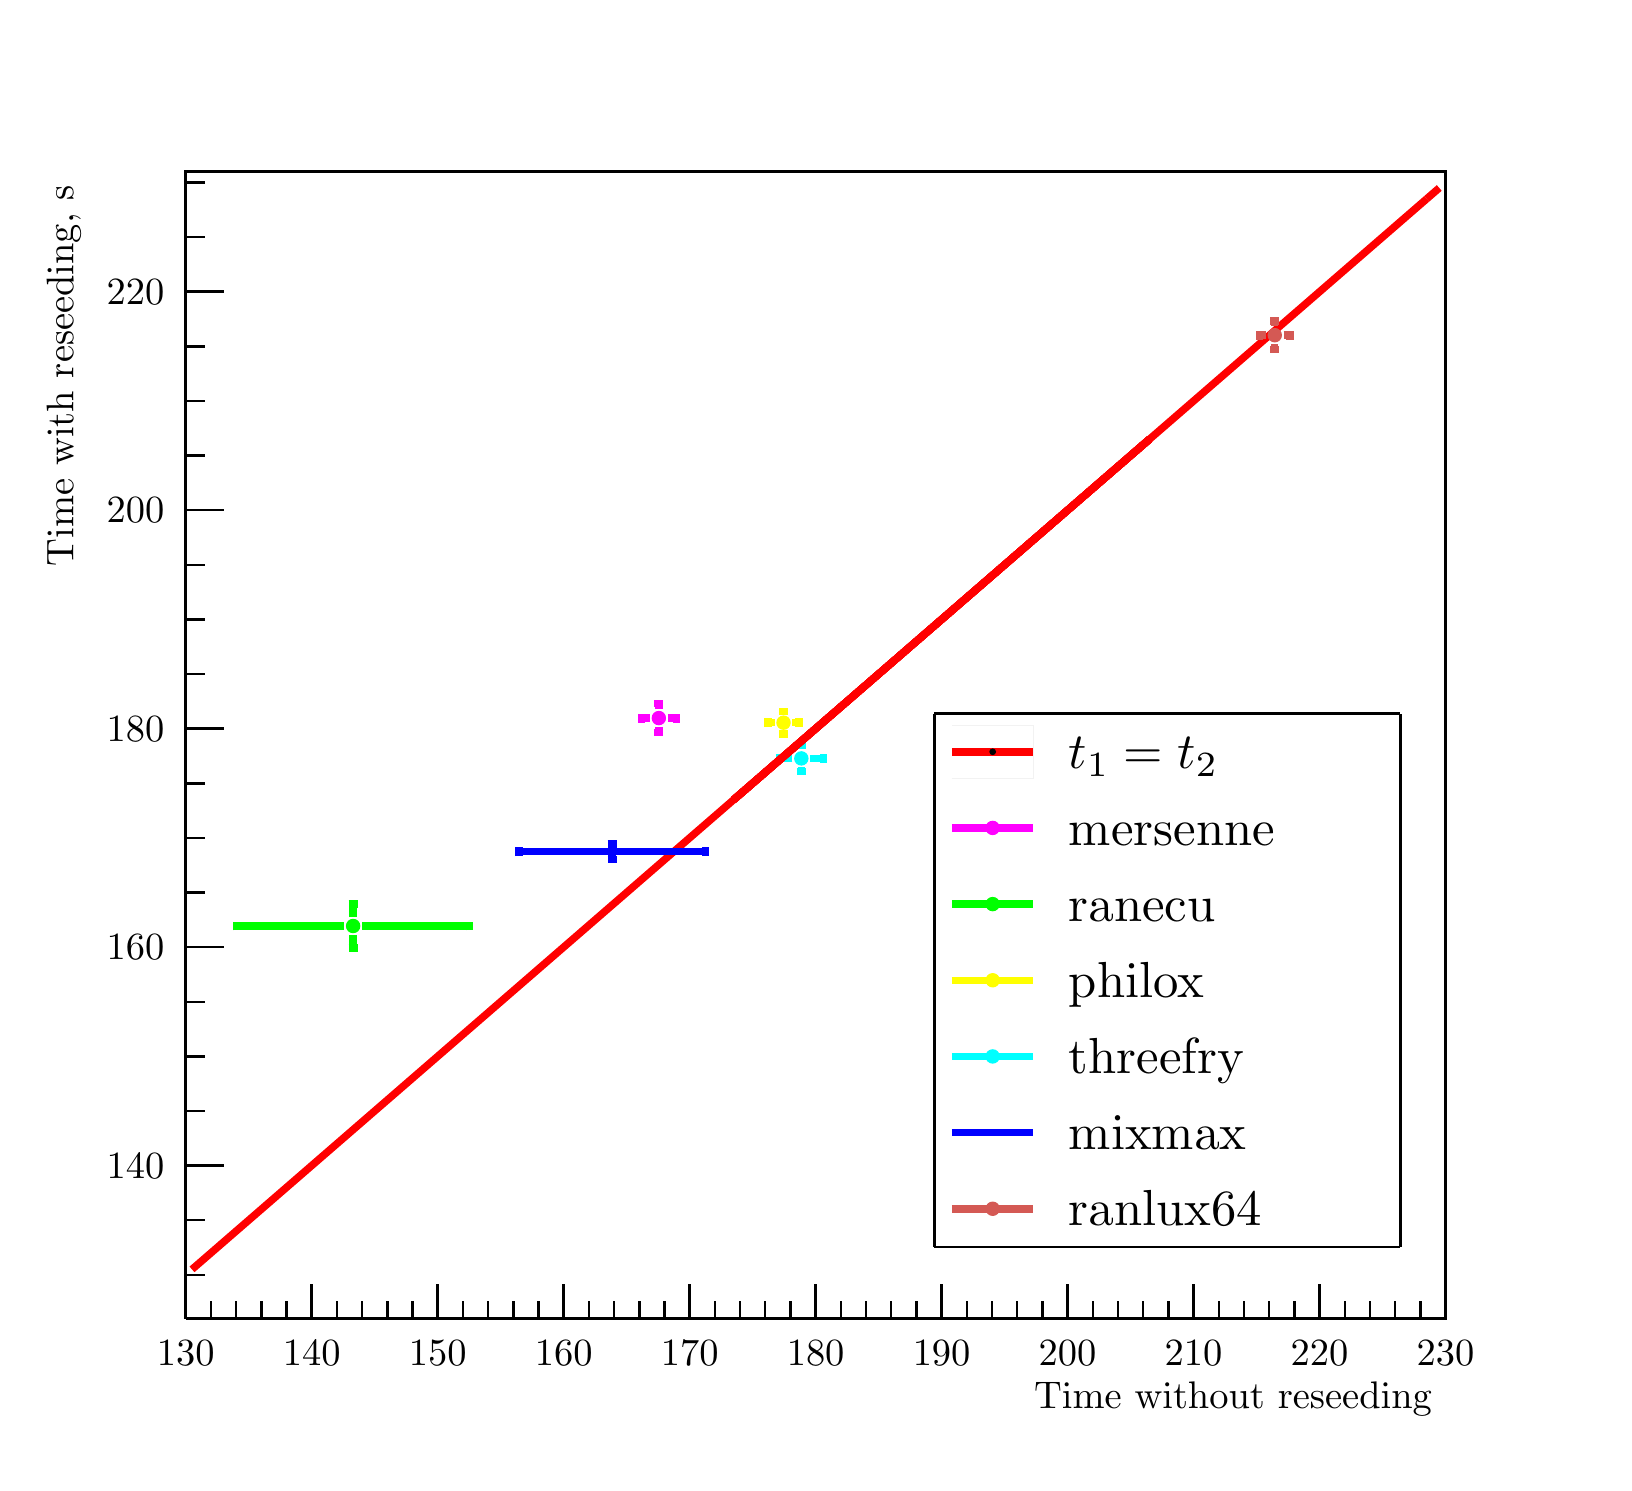
\begin{tikzpicture}
\pgfdeclareplotmark{cross} {
\pgfpathmoveto{\pgfpoint{-0.3\pgfplotmarksize}{\pgfplotmarksize}}
\pgfpathlineto{\pgfpoint{+0.3\pgfplotmarksize}{\pgfplotmarksize}}
\pgfpathlineto{\pgfpoint{+0.3\pgfplotmarksize}{0.3\pgfplotmarksize}}
\pgfpathlineto{\pgfpoint{+1\pgfplotmarksize}{0.3\pgfplotmarksize}}
\pgfpathlineto{\pgfpoint{+1\pgfplotmarksize}{-0.3\pgfplotmarksize}}
\pgfpathlineto{\pgfpoint{+0.3\pgfplotmarksize}{-0.3\pgfplotmarksize}}
\pgfpathlineto{\pgfpoint{+0.3\pgfplotmarksize}{-1.\pgfplotmarksize}}
\pgfpathlineto{\pgfpoint{-0.3\pgfplotmarksize}{-1.\pgfplotmarksize}}
\pgfpathlineto{\pgfpoint{-0.3\pgfplotmarksize}{-0.3\pgfplotmarksize}}
\pgfpathlineto{\pgfpoint{-1.\pgfplotmarksize}{-0.3\pgfplotmarksize}}
\pgfpathlineto{\pgfpoint{-1.\pgfplotmarksize}{0.3\pgfplotmarksize}}
\pgfpathlineto{\pgfpoint{-0.3\pgfplotmarksize}{0.3\pgfplotmarksize}}
\pgfpathclose
\pgfusepathqstroke
}
\pgfdeclareplotmark{cross*} {
\pgfpathmoveto{\pgfpoint{-0.3\pgfplotmarksize}{\pgfplotmarksize}}
\pgfpathlineto{\pgfpoint{+0.3\pgfplotmarksize}{\pgfplotmarksize}}
\pgfpathlineto{\pgfpoint{+0.3\pgfplotmarksize}{0.3\pgfplotmarksize}}
\pgfpathlineto{\pgfpoint{+1\pgfplotmarksize}{0.3\pgfplotmarksize}}
\pgfpathlineto{\pgfpoint{+1\pgfplotmarksize}{-0.3\pgfplotmarksize}}
\pgfpathlineto{\pgfpoint{+0.3\pgfplotmarksize}{-0.3\pgfplotmarksize}}
\pgfpathlineto{\pgfpoint{+0.3\pgfplotmarksize}{-1.\pgfplotmarksize}}
\pgfpathlineto{\pgfpoint{-0.3\pgfplotmarksize}{-1.\pgfplotmarksize}}
\pgfpathlineto{\pgfpoint{-0.3\pgfplotmarksize}{-0.3\pgfplotmarksize}}
\pgfpathlineto{\pgfpoint{-1.\pgfplotmarksize}{-0.3\pgfplotmarksize}}
\pgfpathlineto{\pgfpoint{-1.\pgfplotmarksize}{0.3\pgfplotmarksize}}
\pgfpathlineto{\pgfpoint{-0.3\pgfplotmarksize}{0.3\pgfplotmarksize}}
\pgfpathclose
\pgfusepathqfillstroke
}
\pgfdeclareplotmark{newstar} {
\pgfpathmoveto{\pgfqpoint{0pt}{\pgfplotmarksize}}
\pgfpathlineto{\pgfqpointpolar{44}{0.5\pgfplotmarksize}}
\pgfpathlineto{\pgfqpointpolar{18}{\pgfplotmarksize}}
\pgfpathlineto{\pgfqpointpolar{-20}{0.5\pgfplotmarksize}}
\pgfpathlineto{\pgfqpointpolar{-54}{\pgfplotmarksize}}
\pgfpathlineto{\pgfqpointpolar{-90}{0.5\pgfplotmarksize}}
\pgfpathlineto{\pgfqpointpolar{234}{\pgfplotmarksize}}
\pgfpathlineto{\pgfqpointpolar{198}{0.5\pgfplotmarksize}}
\pgfpathlineto{\pgfqpointpolar{162}{\pgfplotmarksize}}
\pgfpathlineto{\pgfqpointpolar{134}{0.5\pgfplotmarksize}}
\pgfpathclose
\pgfusepathqstroke
}
\pgfdeclareplotmark{newstar*} {
\pgfpathmoveto{\pgfqpoint{0pt}{\pgfplotmarksize}}
\pgfpathlineto{\pgfqpointpolar{44}{0.5\pgfplotmarksize}}
\pgfpathlineto{\pgfqpointpolar{18}{\pgfplotmarksize}}
\pgfpathlineto{\pgfqpointpolar{-20}{0.5\pgfplotmarksize}}
\pgfpathlineto{\pgfqpointpolar{-54}{\pgfplotmarksize}}
\pgfpathlineto{\pgfqpointpolar{-90}{0.5\pgfplotmarksize}}
\pgfpathlineto{\pgfqpointpolar{234}{\pgfplotmarksize}}
\pgfpathlineto{\pgfqpointpolar{198}{0.5\pgfplotmarksize}}
\pgfpathlineto{\pgfqpointpolar{162}{\pgfplotmarksize}}
\pgfpathlineto{\pgfqpointpolar{134}{0.5\pgfplotmarksize}}
\pgfpathclose
\pgfusepathqfillstroke
}
\definecolor{c}{rgb}{1,1,1};
\draw [color=c, fill=c] (0,0) rectangle (20,18.2077);
\draw [color=c, fill=c] (2,1.82077) rectangle (18,16.3869);
\definecolor{c}{rgb}{0,0,0};
\draw [c,line width=0.9] (2,1.82077) -- (2,16.3869) -- (18,16.3869) -- (18,1.82077) -- (2,1.82077);
\definecolor{c}{rgb}{1,1,1};
\draw [color=c, fill=c] (2,1.82077) rectangle (18,16.3869);
\definecolor{c}{rgb}{0,0,0};
\draw [c,line width=0.9] (2,1.82077) -- (2,16.3869) -- (18,16.3869) -- (18,1.82077) -- (2,1.82077);
\definecolor{c}{rgb}{1,0,0};
\draw [c,line width=2.7] (2.08,2.44503) -- (2.24,2.58376) -- (2.4,2.72248) -- (2.56,2.86121) -- (2.72,2.99993) -- (2.88,3.13866) -- (3.04,3.27738) -- (3.2,3.41611) -- (3.36,3.55483) -- (3.52,3.69356) -- (3.68,3.83228) -- (3.84,3.97101) -- (4,4.10973)
 -- (4.16,4.24846) -- (4.32,4.38718) -- (4.48,4.52591) -- (4.64,4.66463) -- (4.8,4.80336) -- (4.96,4.94209) -- (5.12,5.08081) -- (5.28,5.21954) -- (5.44,5.35826) -- (5.6,5.49699) -- (5.76,5.63571) -- (5.92,5.77444) -- (6.08,5.91316) -- (6.24,6.05189)
 -- (6.4,6.19061) -- (6.56,6.32934) -- (6.72,6.46806) -- (6.88,6.60679) -- (7.04,6.74551) -- (7.2,6.88424) -- (7.36,7.02296) -- (7.52,7.16169) -- (7.68,7.30041) -- (7.84,7.43914) -- (8,7.57786) -- (8.16,7.71659) -- (8.32,7.85531) -- (8.48,7.99404) --
 (8.64,8.13276) -- (8.8,8.27149) -- (8.96,8.41021) -- (9.12,8.54894) -- (9.28,8.68766) -- (9.44,8.82639) -- (9.6,8.96512) -- (9.76,9.10384) -- (9.92,9.24257);
\draw [c,line width=2.7] (9.92,9.24257) -- (10.08,9.38129) -- (10.24,9.52002) -- (10.4,9.65874) -- (10.56,9.79747) -- (10.72,9.93619) -- (10.88,10.0749) -- (11.04,10.2136) -- (11.2,10.3524) -- (11.36,10.4911) -- (11.52,10.6298) -- (11.68,10.7685) --
 (11.84,10.9073) -- (12,11.046) -- (12.16,11.1847) -- (12.32,11.3234) -- (12.48,11.4622) -- (12.64,11.6009) -- (12.8,11.7396) -- (12.96,11.8783) -- (13.12,12.0171) -- (13.28,12.1558) -- (13.44,12.2945) -- (13.6,12.4332) -- (13.76,12.572) --
 (13.92,12.7107) -- (14.08,12.8494) -- (14.24,12.9881) -- (14.4,13.1269) -- (14.56,13.2656) -- (14.72,13.4043) -- (14.88,13.543) -- (15.04,13.6818) -- (15.2,13.8205) -- (15.36,13.9592) -- (15.52,14.0979) -- (15.68,14.2367) -- (15.84,14.3754) --
 (16,14.5141) -- (16.16,14.6528) -- (16.32,14.7916) -- (16.48,14.9303) -- (16.64,15.069) -- (16.8,15.2077) -- (16.96,15.3465) -- (17.12,15.4852) -- (17.28,15.6239) -- (17.44,15.7627) -- (17.6,15.9014) -- (17.76,16.0401);
\draw [c,line width=2.7] (17.76,16.0401) -- (17.92,16.1788);
\definecolor{c}{rgb}{0,0,0};
\draw [c,line width=0.9] (2,1.82077) -- (18,1.82077);
\draw [c,line width=0.9] (2,2.25775) -- (2,1.82077);
\draw [c,line width=0.9] (2.32,2.03926) -- (2.32,1.82077);
\draw [c,line width=0.9] (2.64,2.03926) -- (2.64,1.82077);
\draw [c,line width=0.9] (2.96,2.03926) -- (2.96,1.82077);
\draw [c,line width=0.9] (3.28,2.03926) -- (3.28,1.82077);
\draw [c,line width=0.9] (3.6,2.25775) -- (3.6,1.82077);
\draw [c,line width=0.9] (3.92,2.03926) -- (3.92,1.82077);
\draw [c,line width=0.9] (4.24,2.03926) -- (4.24,1.82077);
\draw [c,line width=0.9] (4.56,2.03926) -- (4.56,1.82077);
\draw [c,line width=0.9] (4.88,2.03926) -- (4.88,1.82077);
\draw [c,line width=0.9] (5.2,2.25775) -- (5.2,1.82077);
\draw [c,line width=0.9] (5.52,2.03926) -- (5.52,1.82077);
\draw [c,line width=0.9] (5.84,2.03926) -- (5.84,1.82077);
\draw [c,line width=0.9] (6.16,2.03926) -- (6.16,1.82077);
\draw [c,line width=0.9] (6.48,2.03926) -- (6.48,1.82077);
\draw [c,line width=0.9] (6.8,2.25775) -- (6.8,1.82077);
\draw [c,line width=0.9] (7.12,2.03926) -- (7.12,1.82077);
\draw [c,line width=0.9] (7.44,2.03926) -- (7.44,1.82077);
\draw [c,line width=0.9] (7.76,2.03926) -- (7.76,1.82077);
\draw [c,line width=0.9] (8.08,2.03926) -- (8.08,1.82077);
\draw [c,line width=0.9] (8.4,2.25775) -- (8.4,1.82077);
\draw [c,line width=0.9] (8.72,2.03926) -- (8.72,1.82077);
\draw [c,line width=0.9] (9.04,2.03926) -- (9.04,1.82077);
\draw [c,line width=0.9] (9.36,2.03926) -- (9.36,1.82077);
\draw [c,line width=0.9] (9.68,2.03926) -- (9.68,1.82077);
\draw [c,line width=0.9] (10,2.25775) -- (10,1.82077);
\draw [c,line width=0.9] (10.32,2.03926) -- (10.32,1.82077);
\draw [c,line width=0.9] (10.64,2.03926) -- (10.64,1.82077);
\draw [c,line width=0.9] (10.96,2.03926) -- (10.96,1.82077);
\draw [c,line width=0.9] (11.28,2.03926) -- (11.28,1.82077);
\draw [c,line width=0.9] (11.6,2.25775) -- (11.6,1.82077);
\draw [c,line width=0.9] (11.92,2.03926) -- (11.92,1.82077);
\draw [c,line width=0.9] (12.24,2.03926) -- (12.24,1.82077);
\draw [c,line width=0.9] (12.56,2.03926) -- (12.56,1.82077);
\draw [c,line width=0.9] (12.88,2.03926) -- (12.88,1.82077);
\draw [c,line width=0.9] (13.2,2.25775) -- (13.2,1.82077);
\draw [c,line width=0.9] (13.52,2.03926) -- (13.52,1.82077);
\draw [c,line width=0.9] (13.84,2.03926) -- (13.84,1.82077);
\draw [c,line width=0.9] (14.16,2.03926) -- (14.16,1.82077);
\draw [c,line width=0.9] (14.48,2.03926) -- (14.48,1.82077);
\draw [c,line width=0.9] (14.8,2.25775) -- (14.8,1.82077);
\draw [c,line width=0.9] (15.12,2.03926) -- (15.12,1.82077);
\draw [c,line width=0.9] (15.44,2.03926) -- (15.44,1.82077);
\draw [c,line width=0.9] (15.76,2.03926) -- (15.76,1.82077);
\draw [c,line width=0.9] (16.08,2.03926) -- (16.08,1.82077);
\draw [c,line width=0.9] (16.4,2.25775) -- (16.4,1.82077);
\draw [c,line width=0.9] (16.72,2.03926) -- (16.72,1.82077);
\draw [c,line width=0.9] (17.04,2.03926) -- (17.04,1.82077);
\draw [c,line width=0.9] (17.36,2.03926) -- (17.36,1.82077);
\draw [c,line width=0.9] (17.68,2.03926) -- (17.68,1.82077);
\draw [c,line width=0.9] (18,2.25775) -- (18,1.82077);
\draw [anchor=base] (2,1.21991) node[scale=1.39008, color=c, rotate=0]{130};
\draw [anchor=base] (3.6,1.21991) node[scale=1.39008, color=c, rotate=0]{140};
\draw [anchor=base] (5.2,1.21991) node[scale=1.39008, color=c, rotate=0]{150};
\draw [anchor=base] (6.8,1.21991) node[scale=1.39008, color=c, rotate=0]{160};
\draw [anchor=base] (8.4,1.21991) node[scale=1.39008, color=c, rotate=0]{170};
\draw [anchor=base] (10,1.21991) node[scale=1.39008, color=c, rotate=0]{180};
\draw [anchor=base] (11.6,1.21991) node[scale=1.39008, color=c, rotate=0]{190};
\draw [anchor=base] (13.2,1.21991) node[scale=1.39008, color=c, rotate=0]{200};
\draw [anchor=base] (14.8,1.21991) node[scale=1.39008, color=c, rotate=0]{210};
\draw [anchor=base] (16.4,1.21991) node[scale=1.39008, color=c, rotate=0]{220};
\draw [anchor=base] (18,1.21991) node[scale=1.39008, color=c, rotate=0]{230};
\draw [anchor= east] (18,0.801138) node[scale=1.39008, color=c, rotate=0]{Time without reseeding};
\draw [c,line width=0.9] (2,1.82077) -- (2,16.3869);
\draw [c,line width=0.9] (2.48,3.76292) -- (2,3.76292);
\draw [c,line width=0.9] (2.24,4.45655) -- (2,4.45655);
\draw [c,line width=0.9] (2.24,5.15017) -- (2,5.15017);
\draw [c,line width=0.9] (2.24,5.8438) -- (2,5.8438);
\draw [c,line width=0.9] (2.48,6.53742) -- (2,6.53742);
\draw [c,line width=0.9] (2.24,7.23105) -- (2,7.23105);
\draw [c,line width=0.9] (2.24,7.92468) -- (2,7.92468);
\draw [c,line width=0.9] (2.24,8.6183) -- (2,8.6183);
\draw [c,line width=0.9] (2.48,9.31193) -- (2,9.31193);
\draw [c,line width=0.9] (2.24,10.0056) -- (2,10.0056);
\draw [c,line width=0.9] (2.24,10.6992) -- (2,10.6992);
\draw [c,line width=0.9] (2.24,11.3928) -- (2,11.3928);
\draw [c,line width=0.9] (2.48,12.0864) -- (2,12.0864);
\draw [c,line width=0.9] (2.24,12.7801) -- (2,12.7801);
\draw [c,line width=0.9] (2.24,13.4737) -- (2,13.4737);
\draw [c,line width=0.9] (2.24,14.1673) -- (2,14.1673);
\draw [c,line width=0.9] (2.48,14.8609) -- (2,14.8609);
\draw [c,line width=0.9] (2.48,3.76292) -- (2,3.76292);
\draw [c,line width=0.9] (2.24,3.06929) -- (2,3.06929);
\draw [c,line width=0.9] (2.24,2.37567) -- (2,2.37567);
\draw [c,line width=0.9] (2.48,14.8609) -- (2,14.8609);
\draw [c,line width=0.9] (2.24,15.5546) -- (2,15.5546);
\draw [c,line width=0.9] (2.24,16.2482) -- (2,16.2482);
\draw [anchor= east] (1.9,3.76292) node[scale=1.39008, color=c, rotate=0]{140};
\draw [anchor= east] (1.9,6.53742) node[scale=1.39008, color=c, rotate=0]{160};
\draw [anchor= east] (1.9,9.31193) node[scale=1.39008, color=c, rotate=0]{180};
\draw [anchor= east] (1.9,12.0864) node[scale=1.39008, color=c, rotate=0]{200};
\draw [anchor= east] (1.9,14.8609) node[scale=1.39008, color=c, rotate=0]{220};
\draw [anchor= east] (0.452347,16.3869) node[scale=1.39008, color=c, rotate=90]{Time with reseeding, s};
\definecolor{c}{rgb}{1,0,1};
\draw [c,line width=2.7] (7.895,9.44658) -- (7.7853,9.44658);
\draw [c,line width=2.7] (7.7853,9.38968) -- (7.7853,9.50348);
\draw [c,line width=2.7] (8.1226,9.44658) -- (8.2323,9.44658);
\draw [c,line width=2.7] (8.2323,9.38968) -- (8.2323,9.50348);
\draw [c,line width=2.7] (8.0088,9.56038) -- (8.0088,9.63112);
\draw [c,line width=2.7] (7.9519,9.63112) -- (8.0657,9.63112);
\draw [c,line width=2.7] (8.0088,9.33278) -- (8.0088,9.26204);
\draw [c,line width=2.7] (7.9519,9.26204) -- (8.0657,9.26204);
\foreach \P in {(8.0088,9.44658)}{\draw[mark options={color=c,fill=c},mark size=2.402402pt,mark=*] plot coordinates {\P};}
\definecolor{c}{rgb}{0,1,0};
\draw [c,line width=2.7] (4.0123,6.80586) -- (2.64491,6.80586);
\draw [c,line width=2.7] (2.64491,6.74896) -- (2.64491,6.86276);
\draw [c,line width=2.7] (4.2399,6.80586) -- (5.60729,6.80586);
\draw [c,line width=2.7] (5.60729,6.74896) -- (5.60729,6.86276);
\draw [c,line width=2.7] (4.1261,6.91966) -- (4.1261,7.08758);
\draw [c,line width=2.7] (4.0692,7.08758) -- (4.183,7.08758);
\draw [c,line width=2.7] (4.1261,6.69206) -- (4.1261,6.52414);
\draw [c,line width=2.7] (4.0692,6.52414) -- (4.183,6.52414);
\foreach \P in {(4.1261,6.80586)}{\draw[mark options={color=c,fill=c},mark size=2.402402pt,mark=*] plot coordinates {\P};}
\definecolor{c}{rgb}{1,1,0};
\draw [c,line width=2.7] (9.4785,9.38823) -- (9.3968,9.38823);
\draw [c,line width=2.7] (9.3968,9.33133) -- (9.3968,9.44513);
\draw [c,line width=2.7] (9.7061,9.38823) -- (9.7878,9.38823);
\draw [c,line width=2.7] (9.7878,9.33133) -- (9.7878,9.44513);
\draw [c,line width=2.7] (9.5923,9.50203) -- (9.5923,9.53051);
\draw [c,line width=2.7] (9.5354,9.53051) -- (9.6492,9.53051);
\draw [c,line width=2.7] (9.5923,9.27443) -- (9.5923,9.24595);
\draw [c,line width=2.7] (9.5354,9.24595) -- (9.6492,9.24595);
\foreach \P in {(9.5923,9.38823)}{\draw[mark options={color=c,fill=c},mark size=2.402402pt,mark=*] plot coordinates {\P};}
\definecolor{c}{rgb}{0,1,1};
\draw [c,line width=2.7] (9.7045,8.93434) -- (9.53897,8.93434);
\draw [c,line width=2.7] (9.53897,8.87744) -- (9.53897,8.99123);
\draw [c,line width=2.7] (9.9321,8.93434) -- (10.0976,8.93434);
\draw [c,line width=2.7] (10.0976,8.87744) -- (10.0976,8.99123);
\draw [c,line width=2.7] (9.8183,9.04813) -- (9.8183,9.09913);
\draw [c,line width=2.7] (9.7614,9.09913) -- (9.8752,9.09913);
\draw [c,line width=2.7] (9.8183,8.82054) -- (9.8183,8.76955);
\draw [c,line width=2.7] (9.7614,8.76955) -- (9.8752,8.76955);
\foreach \P in {(9.8183,8.93434)}{\draw[mark options={color=c,fill=c},mark size=2.402402pt,mark=*] plot coordinates {\P};}
\definecolor{c}{rgb}{0,0,1};
\draw [c,line width=2.7] (7.4154,7.74919) -- (6.23044,7.74919);
\draw [c,line width=2.7] (6.23044,7.69229) -- (6.23044,7.80609);
\draw [c,line width=2.7] (7.4154,7.74919) -- (8.60036,7.74919);
\draw [c,line width=2.7] (8.60036,7.69229) -- (8.60036,7.80609);
\draw [c,line width=2.7] (7.4154,7.74919) -- (7.4154,7.84836);
\draw [c,line width=2.7] (7.3585,7.84836) -- (7.4723,7.84836);
\draw [c,line width=2.7] (7.4154,7.74919) -- (7.4154,7.65002);
\draw [c,line width=2.7] (7.3585,7.65002) -- (7.4723,7.65002);
\foreach \P in {(7.4154,7.74919)}{\draw[mark options={color=c,fill=c},mark size=2.402402pt,mark=] plot coordinates {\P};}
\definecolor{c}{rgb}{0.83,0.35,0.33};
\draw [c,line width=2.7] (15.717,14.3089) -- (15.6367,14.3089);
\draw [c,line width=2.7] (15.6367,14.252) -- (15.6367,14.3658);
\draw [c,line width=2.7] (15.9446,14.3089) -- (16.0249,14.3089);
\draw [c,line width=2.7] (16.0249,14.252) -- (16.0249,14.3658);
\draw [c,line width=2.7] (15.8308,14.4227) -- (15.8308,14.4883);
\draw [c,line width=2.7] (15.7739,14.4883) -- (15.8877,14.4883);
\draw [c,line width=2.7] (15.8308,14.1951) -- (15.8308,14.1295);
\draw [c,line width=2.7] (15.7739,14.1295) -- (15.8877,14.1295);
\foreach \P in {(15.8308,14.3089)}{\draw[mark options={color=c,fill=c},mark size=2.402402pt,mark=*] plot coordinates {\P};}
\definecolor{c}{rgb}{1,1,1};
\draw [color=c, fill=c] (11.5089,2.73115) rectangle (17.426,9.50213);
\definecolor{c}{rgb}{0,0,0};
\draw [c,line width=0.9] (11.5089,2.73115) -- (17.426,2.73115);
\draw [c,line width=0.9] (17.426,2.73115) -- (17.426,9.50213);
\draw [c,line width=0.9] (17.426,9.50213) -- (11.5089,9.50213);
\draw [c,line width=0.9] (11.5089,9.50213) -- (11.5089,2.73115);
\draw [anchor=base west] (12.9882,8.80085) node[scale=1.83238, color=c, rotate=0]{$t_{1} = t_{2}$};
\definecolor{c}{rgb}{0.95,0.95,0.95};
\draw [c] (11.7308,8.67994) -- (12.7663,8.67994) -- (12.7663,9.35704) -- (11.7308,9.35704);
\definecolor{c}{rgb}{1,0,0};
\draw [c,line width=2.7] (11.7308,9.01849) -- (12.7663,9.01849);
\definecolor{c}{rgb}{0,0,0};
\foreach \P in {(12.2485,9.01849)}{\draw[mark options={color=c,fill=c},mark size=2.402402pt,mark=*,mark size=1pt] plot coordinates {\P};}
\draw [anchor=base west] (12.9882,7.83357) node[scale=1.83238, color=c, rotate=0]{mersenne};
\definecolor{c}{rgb}{1,1,1};
\draw [c] (11.7308,7.71266) -- (12.7663,7.71266) -- (12.7663,8.38976) -- (11.7308,8.38976);
\definecolor{c}{rgb}{1,0,1};
\draw [c,line width=2.7] (11.7308,8.05121) -- (12.7663,8.05121);
\foreach \P in {(12.2485,8.05121)}{\draw[mark options={color=c,fill=c},mark size=2.402402pt,mark=*] plot coordinates {\P};}
\definecolor{c}{rgb}{0,0,0};
\draw [anchor=base west] (12.9882,6.86629) node[scale=1.83238, color=c, rotate=0]{ranecu};
\definecolor{c}{rgb}{1,1,1};
\draw [c] (11.7308,6.74538) -- (12.7663,6.74538) -- (12.7663,7.42248) -- (11.7308,7.42248);
\definecolor{c}{rgb}{0,1,0};
\draw [c,line width=2.7] (11.7308,7.08393) -- (12.7663,7.08393);
\foreach \P in {(12.2485,7.08393)}{\draw[mark options={color=c,fill=c},mark size=2.402402pt,mark=*] plot coordinates {\P};}
\definecolor{c}{rgb}{0,0,0};
\draw [anchor=base west] (12.9882,5.899) node[scale=1.83238, color=c, rotate=0]{philox};
\definecolor{c}{rgb}{1,1,1};
\draw [c] (11.7308,5.77809) -- (12.7663,5.77809) -- (12.7663,6.45519) -- (11.7308,6.45519);
\definecolor{c}{rgb}{1,1,0};
\draw [c,line width=2.7] (11.7308,6.11664) -- (12.7663,6.11664);
\foreach \P in {(12.2485,6.11664)}{\draw[mark options={color=c,fill=c},mark size=2.402402pt,mark=*] plot coordinates {\P};}
\definecolor{c}{rgb}{0,0,0};
\draw [anchor=base west] (12.9882,4.93172) node[scale=1.83238, color=c, rotate=0]{threefry};
\definecolor{c}{rgb}{1,1,1};
\draw [c] (11.7308,4.81081) -- (12.7663,4.81081) -- (12.7663,5.48791) -- (11.7308,5.48791);
\definecolor{c}{rgb}{0,1,1};
\draw [c,line width=2.7] (11.7308,5.14936) -- (12.7663,5.14936);
\foreach \P in {(12.2485,5.14936)}{\draw[mark options={color=c,fill=c},mark size=2.402402pt,mark=*] plot coordinates {\P};}
\definecolor{c}{rgb}{0,0,0};
\draw [anchor=base west] (12.9882,3.96444) node[scale=1.83238, color=c, rotate=0]{mixmax};
\definecolor{c}{rgb}{1,1,1};
\draw [c] (11.7308,3.84353) -- (12.7663,3.84353) -- (12.7663,4.52063) -- (11.7308,4.52063);
\definecolor{c}{rgb}{0,0,1};
\draw [c,line width=2.7] (11.7308,4.18208) -- (12.7663,4.18208);
\foreach \P in {(12.2485,4.18208)}{\draw[mark options={color=c,fill=c},mark size=2.402402pt,mark=] plot coordinates {\P};}
\definecolor{c}{rgb}{0,0,0};
\draw [anchor=base west] (12.9882,2.99716) node[scale=1.83238, color=c, rotate=0]{ranlux64};
\definecolor{c}{rgb}{1,1,1};
\draw [c] (11.7308,2.87624) -- (12.7663,2.87624) -- (12.7663,3.55334) -- (11.7308,3.55334);
\definecolor{c}{rgb}{0.83,0.35,0.33};
\draw [c,line width=2.7] (11.7308,3.21479) -- (12.7663,3.21479);
\foreach \P in {(12.2485,3.21479)}{\draw[mark options={color=c,fill=c},mark size=2.402402pt,mark=*] plot coordinates {\P};}
\definecolor{c}{rgb}{1,0,0};
\draw [c,line width=2.7] (8.96,8.41021) -- (9.01333,8.45646) -- (9.06667,8.5027) -- (9.12,8.54894) -- (9.17333,8.59518) -- (9.22667,8.64142) -- (9.28,8.68766) -- (9.33333,8.73391) -- (9.38667,8.78015) -- (9.44,8.82639) -- (9.49333,8.87263) --
 (9.54667,8.91887) -- (9.6,8.96512) -- (9.65333,9.01136) -- (9.70667,9.0576) -- (9.76,9.10384) -- (9.81333,9.15008) -- (9.86667,9.19632) -- (9.92,9.24257) -- (9.97333,9.28881) -- (10.0267,9.33505) -- (10.08,9.38129) -- (10.1333,9.42753) --
 (10.1867,9.47377) -- (10.24,9.52002) -- (10.2933,9.56626) -- (10.3467,9.6125) -- (10.4,9.65874) -- (10.4533,9.70498) -- (10.5067,9.75123) -- (10.56,9.79747) -- (10.6133,9.84371) -- (10.6667,9.88995) -- (10.72,9.93619) -- (10.7733,9.98243) --
 (10.8267,10.0287) -- (10.88,10.0749) -- (10.9333,10.1212) -- (10.9867,10.1674) -- (11.04,10.2136) -- (11.0933,10.2599) -- (11.1467,10.3061) -- (11.2,10.3524) -- (11.2533,10.3986) -- (11.3067,10.4449) -- (11.36,10.4911) -- (11.4133,10.5373) --
 (11.4667,10.5836) -- (11.52,10.6298) -- (11.5733,10.6761);
\draw [c,line width=2.7] (11.5733,10.6761) -- (11.6267,10.7223) -- (11.68,10.7685) -- (11.7333,10.8148) -- (11.7867,10.861) -- (11.84,10.9073) -- (11.8933,10.9535) -- (11.9467,10.9998) -- (12,11.046) -- (12.0533,11.0922) -- (12.1067,11.1385) --
 (12.16,11.1847) -- (12.2133,11.231) -- (12.2667,11.2772) -- (12.32,11.3234) -- (12.3733,11.3697) -- (12.4267,11.4159) -- (12.48,11.4622) -- (12.5333,11.5084) -- (12.5867,11.5547) -- (12.64,11.6009) -- (12.6933,11.6471) -- (12.7467,11.6934) --
 (12.8,11.7396) -- (12.8533,11.7859) -- (12.9067,11.8321) -- (12.96,11.8783) -- (13.0133,11.9246) -- (13.0667,11.9708) -- (13.12,12.0171) -- (13.1733,12.0633) -- (13.2267,12.1096) -- (13.28,12.1558) -- (13.3333,12.202) -- (13.3867,12.2483) --
 (13.44,12.2945) -- (13.4933,12.3408) -- (13.5467,12.387) -- (13.6,12.4332) -- (13.6533,12.4795) -- (13.7067,12.5257) -- (13.76,12.572) -- (13.8133,12.6182) -- (13.8667,12.6645) -- (13.92,12.7107) -- (13.9733,12.7569) -- (14.0267,12.8032) --
 (14.08,12.8494) -- (14.1333,12.8957) -- (14.1867,12.9419);
\draw [c,line width=2.7] (14.1867,12.9419) -- (14.24,12.9881);
\draw [c,line width=2.7] (8.96,8.41021) -- (9.01333,8.45646) -- (9.06667,8.5027) -- (9.12,8.54894) -- (9.17333,8.59518) -- (9.22667,8.64142) -- (9.28,8.68766) -- (9.33333,8.73391) -- (9.38667,8.78015) -- (9.44,8.82639) -- (9.49333,8.87263) --
 (9.54667,8.91887) -- (9.6,8.96512) -- (9.65333,9.01136) -- (9.70667,9.0576) -- (9.76,9.10384) -- (9.81333,9.15008) -- (9.86667,9.19632) -- (9.92,9.24257) -- (9.97333,9.28881) -- (10.0267,9.33505) -- (10.08,9.38129) -- (10.1333,9.42753) --
 (10.1867,9.47377) -- (10.24,9.52002) -- (10.2933,9.56626) -- (10.3467,9.6125) -- (10.4,9.65874) -- (10.4533,9.70498) -- (10.5067,9.75123) -- (10.56,9.79747) -- (10.6133,9.84371) -- (10.6667,9.88995) -- (10.72,9.93619) -- (10.7733,9.98243) --
 (10.8267,10.0287) -- (10.88,10.0749) -- (10.9333,10.1212) -- (10.9867,10.1674) -- (11.04,10.2136) -- (11.0933,10.2599) -- (11.1467,10.3061) -- (11.2,10.3524) -- (11.2533,10.3986) -- (11.3067,10.4449) -- (11.36,10.4911) -- (11.4133,10.5373) --
 (11.4667,10.5836) -- (11.52,10.6298) -- (11.5733,10.6761);
\draw [c,line width=2.7] (11.5733,10.6761) -- (11.6267,10.7223) -- (11.68,10.7685) -- (11.7333,10.8148) -- (11.7867,10.861) -- (11.84,10.9073) -- (11.8933,10.9535) -- (11.9467,10.9998) -- (12,11.046) -- (12.0533,11.0922) -- (12.1067,11.1385) --
 (12.16,11.1847) -- (12.2133,11.231) -- (12.2667,11.2772) -- (12.32,11.3234) -- (12.3733,11.3697) -- (12.4267,11.4159) -- (12.48,11.4622) -- (12.5333,11.5084) -- (12.5867,11.5547) -- (12.64,11.6009) -- (12.6933,11.6471) -- (12.7467,11.6934) --
 (12.8,11.7396) -- (12.8533,11.7859) -- (12.9067,11.8321) -- (12.96,11.8783) -- (13.0133,11.9246) -- (13.0667,11.9708) -- (13.12,12.0171) -- (13.1733,12.0633) -- (13.2267,12.1096) -- (13.28,12.1558) -- (13.3333,12.202) -- (13.3867,12.2483) --
 (13.44,12.2945) -- (13.4933,12.3408) -- (13.5467,12.387) -- (13.6,12.4332) -- (13.6533,12.4795) -- (13.7067,12.5257) -- (13.76,12.572) -- (13.8133,12.6182) -- (13.8667,12.6645) -- (13.92,12.7107) -- (13.9733,12.7569) -- (14.0267,12.8032) --
 (14.08,12.8494) -- (14.1333,12.8957) -- (14.1867,12.9419);
\draw [c,line width=2.7] (14.1867,12.9419) -- (14.24,12.9881);
\draw [c,line width=2.7] (8.96,8.41021) -- (9.01333,8.45646) -- (9.06667,8.5027) -- (9.12,8.54894) -- (9.17333,8.59518) -- (9.22667,8.64142) -- (9.28,8.68766) -- (9.33333,8.73391) -- (9.38667,8.78015) -- (9.44,8.82639) -- (9.49333,8.87263) --
 (9.54667,8.91887) -- (9.6,8.96512) -- (9.65333,9.01136) -- (9.70667,9.0576) -- (9.76,9.10384) -- (9.81333,9.15008) -- (9.86667,9.19632) -- (9.92,9.24257) -- (9.97333,9.28881) -- (10.0267,9.33505) -- (10.08,9.38129) -- (10.1333,9.42753) --
 (10.1867,9.47377) -- (10.24,9.52002) -- (10.2933,9.56626) -- (10.3467,9.6125) -- (10.4,9.65874) -- (10.4533,9.70498) -- (10.5067,9.75123) -- (10.56,9.79747) -- (10.6133,9.84371) -- (10.6667,9.88995) -- (10.72,9.93619) -- (10.7733,9.98243) --
 (10.8267,10.0287) -- (10.88,10.0749) -- (10.9333,10.1212) -- (10.9867,10.1674) -- (11.04,10.2136) -- (11.0933,10.2599) -- (11.1467,10.3061) -- (11.2,10.3524) -- (11.2533,10.3986) -- (11.3067,10.4449) -- (11.36,10.4911) -- (11.4133,10.5373) --
 (11.4667,10.5836) -- (11.52,10.6298) -- (11.5733,10.6761);
\draw [c,line width=2.7] (11.5733,10.6761) -- (11.6267,10.7223) -- (11.68,10.7685) -- (11.7333,10.8148) -- (11.7867,10.861) -- (11.84,10.9073) -- (11.8933,10.9535) -- (11.9467,10.9998) -- (12,11.046) -- (12.0533,11.0922) -- (12.1067,11.1385) --
 (12.16,11.1847) -- (12.2133,11.231) -- (12.2667,11.2772) -- (12.32,11.3234) -- (12.3733,11.3697) -- (12.4267,11.4159) -- (12.48,11.4622) -- (12.5333,11.5084) -- (12.5867,11.5547) -- (12.64,11.6009) -- (12.6933,11.6471) -- (12.7467,11.6934) --
 (12.8,11.7396) -- (12.8533,11.7859) -- (12.9067,11.8321) -- (12.96,11.8783) -- (13.0133,11.9246) -- (13.0667,11.9708) -- (13.12,12.0171) -- (13.1733,12.0633) -- (13.2267,12.1096) -- (13.28,12.1558) -- (13.3333,12.202) -- (13.3867,12.2483) --
 (13.44,12.2945) -- (13.4933,12.3408) -- (13.5467,12.387) -- (13.6,12.4332) -- (13.6533,12.4795) -- (13.7067,12.5257) -- (13.76,12.572) -- (13.8133,12.6182) -- (13.8667,12.6645) -- (13.92,12.7107) -- (13.9733,12.7569) -- (14.0267,12.8032) --
 (14.08,12.8494) -- (14.1333,12.8957) -- (14.1867,12.9419);
\draw [c,line width=2.7] (14.1867,12.9419) -- (14.24,12.9881);
\draw [c,line width=2.7] (8.96,8.41021) -- (9.01333,8.45646) -- (9.06667,8.5027) -- (9.12,8.54894) -- (9.17333,8.59518) -- (9.22667,8.64142) -- (9.28,8.68766) -- (9.33333,8.73391) -- (9.38667,8.78015) -- (9.44,8.82639) -- (9.49333,8.87263) --
 (9.54667,8.91887) -- (9.6,8.96512) -- (9.65333,9.01136) -- (9.70667,9.0576) -- (9.76,9.10384) -- (9.81333,9.15008) -- (9.86667,9.19632) -- (9.92,9.24257) -- (9.97333,9.28881) -- (10.0267,9.33505) -- (10.08,9.38129) -- (10.1333,9.42753) --
 (10.1867,9.47377) -- (10.24,9.52002) -- (10.2933,9.56626) -- (10.3467,9.6125) -- (10.4,9.65874) -- (10.4533,9.70498) -- (10.5067,9.75123) -- (10.56,9.79747) -- (10.6133,9.84371) -- (10.6667,9.88995) -- (10.72,9.93619) -- (10.7733,9.98243) --
 (10.8267,10.0287) -- (10.88,10.0749) -- (10.9333,10.1212) -- (10.9867,10.1674) -- (11.04,10.2136) -- (11.0933,10.2599) -- (11.1467,10.3061) -- (11.2,10.3524) -- (11.2533,10.3986) -- (11.3067,10.4449) -- (11.36,10.4911) -- (11.4133,10.5373) --
 (11.4667,10.5836) -- (11.52,10.6298) -- (11.5733,10.6761);
\draw [c,line width=2.7] (11.5733,10.6761) -- (11.6267,10.7223) -- (11.68,10.7685) -- (11.7333,10.8148) -- (11.7867,10.861) -- (11.84,10.9073) -- (11.8933,10.9535) -- (11.9467,10.9998) -- (12,11.046) -- (12.0533,11.0922) -- (12.1067,11.1385) --
 (12.16,11.1847) -- (12.2133,11.231) -- (12.2667,11.2772) -- (12.32,11.3234) -- (12.3733,11.3697) -- (12.4267,11.4159) -- (12.48,11.4622) -- (12.5333,11.5084) -- (12.5867,11.5547) -- (12.64,11.6009) -- (12.6933,11.6471) -- (12.7467,11.6934) --
 (12.8,11.7396) -- (12.8533,11.7859) -- (12.9067,11.8321) -- (12.96,11.8783) -- (13.0133,11.9246) -- (13.0667,11.9708) -- (13.12,12.0171) -- (13.1733,12.0633) -- (13.2267,12.1096) -- (13.28,12.1558) -- (13.3333,12.202) -- (13.3867,12.2483) --
 (13.44,12.2945) -- (13.4933,12.3408) -- (13.5467,12.387) -- (13.6,12.4332) -- (13.6533,12.4795) -- (13.7067,12.5257) -- (13.76,12.572) -- (13.8133,12.6182) -- (13.8667,12.6645) -- (13.92,12.7107) -- (13.9733,12.7569) -- (14.0267,12.8032) --
 (14.08,12.8494) -- (14.1333,12.8957) -- (14.1867,12.9419);
\draw [c,line width=2.7] (14.1867,12.9419) -- (14.24,12.9881);
\draw [c,line width=2.7] (8.96,8.41021) -- (9.01333,8.45646) -- (9.06667,8.5027) -- (9.12,8.54894) -- (9.17333,8.59518) -- (9.22667,8.64142) -- (9.28,8.68766) -- (9.33333,8.73391) -- (9.38667,8.78015) -- (9.44,8.82639) -- (9.49333,8.87263) --
 (9.54667,8.91887) -- (9.6,8.96512) -- (9.65333,9.01136) -- (9.70667,9.0576) -- (9.76,9.10384) -- (9.81333,9.15008) -- (9.86667,9.19632) -- (9.92,9.24257) -- (9.97333,9.28881) -- (10.0267,9.33505) -- (10.08,9.38129) -- (10.1333,9.42753) --
 (10.1867,9.47377) -- (10.24,9.52002) -- (10.2933,9.56626) -- (10.3467,9.6125) -- (10.4,9.65874) -- (10.4533,9.70498) -- (10.5067,9.75123) -- (10.56,9.79747) -- (10.6133,9.84371) -- (10.6667,9.88995) -- (10.72,9.93619) -- (10.7733,9.98243) --
 (10.8267,10.0287) -- (10.88,10.0749) -- (10.9333,10.1212) -- (10.9867,10.1674) -- (11.04,10.2136) -- (11.0933,10.2599) -- (11.1467,10.3061) -- (11.2,10.3524) -- (11.2533,10.3986) -- (11.3067,10.4449) -- (11.36,10.4911) -- (11.4133,10.5373) --
 (11.4667,10.5836) -- (11.52,10.6298) -- (11.5733,10.6761);
\draw [c,line width=2.7] (11.5733,10.6761) -- (11.6267,10.7223) -- (11.68,10.7685) -- (11.7333,10.8148) -- (11.7867,10.861) -- (11.84,10.9073) -- (11.8933,10.9535) -- (11.9467,10.9998) -- (12,11.046) -- (12.0533,11.0922) -- (12.1067,11.1385) --
 (12.16,11.1847) -- (12.2133,11.231) -- (12.2667,11.2772) -- (12.32,11.3234) -- (12.3733,11.3697) -- (12.4267,11.4159) -- (12.48,11.4622) -- (12.5333,11.5084) -- (12.5867,11.5547) -- (12.64,11.6009) -- (12.6933,11.6471) -- (12.7467,11.6934) --
 (12.8,11.7396) -- (12.8533,11.7859) -- (12.9067,11.8321) -- (12.96,11.8783) -- (13.0133,11.9246) -- (13.0667,11.9708) -- (13.12,12.0171) -- (13.1733,12.0633) -- (13.2267,12.1096) -- (13.28,12.1558) -- (13.3333,12.202) -- (13.3867,12.2483) --
 (13.44,12.2945) -- (13.4933,12.3408) -- (13.5467,12.387) -- (13.6,12.4332) -- (13.6533,12.4795) -- (13.7067,12.5257) -- (13.76,12.572) -- (13.8133,12.6182) -- (13.8667,12.6645) -- (13.92,12.7107) -- (13.9733,12.7569) -- (14.0267,12.8032) --
 (14.08,12.8494) -- (14.1333,12.8957) -- (14.1867,12.9419);
\draw [c,line width=2.7] (14.1867,12.9419) -- (14.24,12.9881);
\draw [c,line width=2.7] (8.96,8.41021) -- (9.01333,8.45646) -- (9.06667,8.5027) -- (9.12,8.54894) -- (9.17333,8.59518) -- (9.22667,8.64142) -- (9.28,8.68766) -- (9.33333,8.73391) -- (9.38667,8.78015) -- (9.44,8.82639) -- (9.49333,8.87263) --
 (9.54667,8.91887) -- (9.6,8.96512) -- (9.65333,9.01136) -- (9.70667,9.0576) -- (9.76,9.10384) -- (9.81333,9.15008) -- (9.86667,9.19632) -- (9.92,9.24257) -- (9.97333,9.28881) -- (10.0267,9.33505) -- (10.08,9.38129) -- (10.1333,9.42753) --
 (10.1867,9.47377) -- (10.24,9.52002) -- (10.2933,9.56626) -- (10.3467,9.6125) -- (10.4,9.65874) -- (10.4533,9.70498) -- (10.5067,9.75123) -- (10.56,9.79747) -- (10.6133,9.84371) -- (10.6667,9.88995) -- (10.72,9.93619) -- (10.7733,9.98243) --
 (10.8267,10.0287) -- (10.88,10.0749) -- (10.9333,10.1212) -- (10.9867,10.1674) -- (11.04,10.2136) -- (11.0933,10.2599) -- (11.1467,10.3061) -- (11.2,10.3524) -- (11.2533,10.3986) -- (11.3067,10.4449) -- (11.36,10.4911) -- (11.4133,10.5373) --
 (11.4667,10.5836) -- (11.52,10.6298) -- (11.5733,10.6761);
\draw [c,line width=2.7] (11.5733,10.6761) -- (11.6267,10.7223) -- (11.68,10.7685) -- (11.7333,10.8148) -- (11.7867,10.861) -- (11.84,10.9073) -- (11.8933,10.9535) -- (11.9467,10.9998) -- (12,11.046) -- (12.0533,11.0922) -- (12.1067,11.1385) --
 (12.16,11.1847) -- (12.2133,11.231) -- (12.2667,11.2772) -- (12.32,11.3234) -- (12.3733,11.3697) -- (12.4267,11.4159) -- (12.48,11.4622) -- (12.5333,11.5084) -- (12.5867,11.5547) -- (12.64,11.6009) -- (12.6933,11.6471) -- (12.7467,11.6934) --
 (12.8,11.7396) -- (12.8533,11.7859) -- (12.9067,11.8321) -- (12.96,11.8783) -- (13.0133,11.9246) -- (13.0667,11.9708) -- (13.12,12.0171) -- (13.1733,12.0633) -- (13.2267,12.1096) -- (13.28,12.1558) -- (13.3333,12.202) -- (13.3867,12.2483) --
 (13.44,12.2945) -- (13.4933,12.3408) -- (13.5467,12.387) -- (13.6,12.4332) -- (13.6533,12.4795) -- (13.7067,12.5257) -- (13.76,12.572) -- (13.8133,12.6182) -- (13.8667,12.6645) -- (13.92,12.7107) -- (13.9733,12.7569) -- (14.0267,12.8032) --
 (14.08,12.8494) -- (14.1333,12.8957) -- (14.1867,12.9419);
\draw [c,line width=2.7] (14.1867,12.9419) -- (14.24,12.9881);
\end{tikzpicture}
}
   \label{USERTIME}
   \caption{User run time with (Y axis) and without (X axis) reseeding.}
  \end{figure}
  
  Figure~\ref{USERTIME} shows run times of a standard geant4 example with the standard random number generation and with reseeding based on pedigrees for different random number generators.
  The overhead depends on the complexity of the seeding function of the random number generator.
  It is the small for the new counter-based generators,
  because the complexity is shifted to the output function.
    
 \section*{ Conclusion }
 
  We implemented reproducible pseudo-random number generation in a Geant4-based prototype.
  We showed the reproducibility of the results independent of the track processing order.
  Also we profiled the overhead for different random number engines.
  We showed that it is rather low for appropriate random number engines.
  
  Therefore it is worth to apply a similar algorithm for reproducible pseudo-random number generation in multithreaded GeantV simulations.
 
 \section*{ Acknowledgements }
 
  Development sponsored by Google in Google Summer of Code 2017 under supervision of John Apostolakis and Sandro Wenzel.
 
 \section*{ Links }
 
  \href{https://bitbucket.org/sd57/pedigree-git}{Standalone prototype}\\
  \href{https://bitbucket.org/sd57/geant4/branch/pedigree}{Geant4-based prototype}\\
  \href{https://sd57.github.io/g4dprng/gsocPreprint.html}{Preprint} about the Geant4-based prototype\\
  \href{https://sd57.github.io/g4dprng/gsoc-proposal-Savin.html}{GSoC proposal}\\
  
%  \newpage
%  \bibliographystyle{plain}
%  \bibliography{gsocReport}
 
\end{document}
